\XeTeXlinebreaklocale "zh"
\XeTeXlinebreakskip = 0pt plus 1pt

\documentclass[11pt,a4paper]{article}

\usepackage{xltxtra,fontspec,xunicode}
\usepackage{amsthm, amsmath, amssymb, amsfonts}
\usepackage{abstract}
\usepackage{subcaption}
\usepackage{graphicx,float} 
\usepackage{minted}

\defaultfontfeatures{Mapping=tex-text,Scale=MatchLowercase}
\setmainfont{DejaVu Serif}
\setsansfont{DejaVu Sans}
\setmonofont{DejaVu Sans Mono}
\usepackage[slantfont,boldfont]{xeCJK} % 允许斜体和粗体
\setCJKmainfont{WenQuanYi Zen Hei}
\setCJKsansfont{WenQuanYi Zen Hei}
\setCJKmonofont{WenQuanYi Zen Hei Mono}

\usepackage{titling}

\renewcommand\refname{参考文献} 

\title{Sudoku的功能及其实现}
\author{miskcoo}

\begin{document}
\maketitle
\section{简介}
Sudoku是一款利用Qt实现的数独游戏,提供了多达10个难度的关卡选择,同时还有丰富的功能来帮助玩家更加高效地求解数独问题,例如候选数、高亮相同数字、高亮选中的行列、撤销当前操作以及提示等功能。玩家还可以手动输入数独题目利用Sudoku帮助求解。

除了传统$9 \times 9$的数独游戏以外,还提供了更高难度的$16 \times 16$的数独游戏。

\begin{figure}[H]
	\centering
	\begin{subfigure}{.45\textwidth}
		\centering
		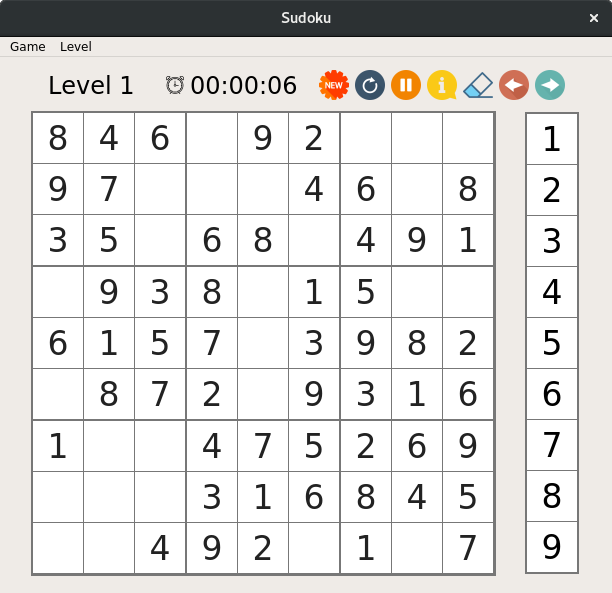
\includegraphics[width=\linewidth]{sudoku-3a.png}
	\end{subfigure}
	\hfill
	\begin{subfigure}{.45\textwidth}
		\centering
		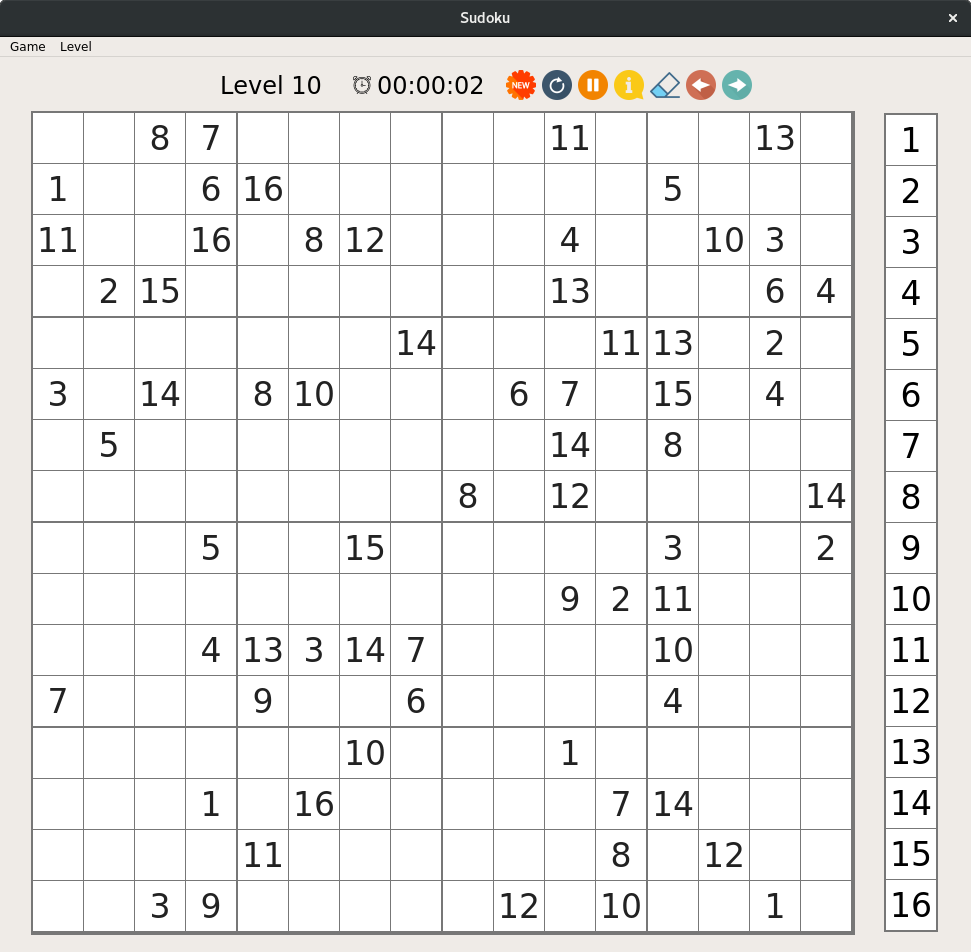
\includegraphics[width=\linewidth]{sudoku-4a.png}
	\end{subfigure}
	\caption{传统的$9\times 9$数独以及高难度的$16\times 16$数独}
\end{figure}

\section{功能}
Sudoku提供了多个方便的按钮:
\begin{itemize}
	\item \textbf{新游戏}:玩家可以开始一局新的游戏。
	\item \textbf{重玩}:玩家可以重新开始本局游戏。
	\item \textbf{暂停}:玩家可以暂停该局游戏(即暂停计时)。
	\item \textbf{提示}:如果当前已经确定的数都是正确的,玩家将会得到一个未填空格的正确数字;如果当前已经确定的数和答案矛盾,导致整个数独无解,那么所有与答案矛盾的数字将会被粗体标出。
	\item \textbf{清除}:清除当前选中格子的所有数字。
	\item \textbf{撤销}:撤销前一步的操作,以及取消撤销(最多可支持50步撤销)。
\end{itemize}

同时可以通过菜单来实现多达10种难度的游戏选择,可以求解任意用户输入的数独问题。

\begin{figure}[H]
	\centering
	\begin{subfigure}{.45\textwidth}
		\centering
		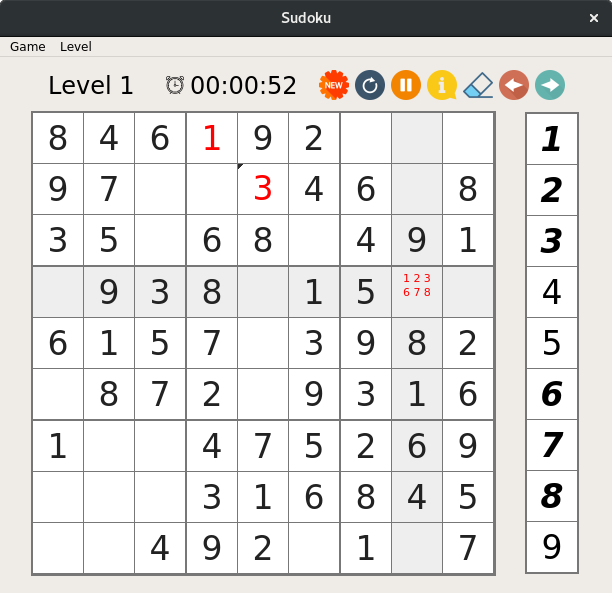
\includegraphics[width=\linewidth]{sudoku-3b.png}
		\caption{最低难度的数独} \label{fig:sudoku-3b}
	\end{subfigure}
	\hfill
	\begin{subfigure}{.45\textwidth}
		\centering
		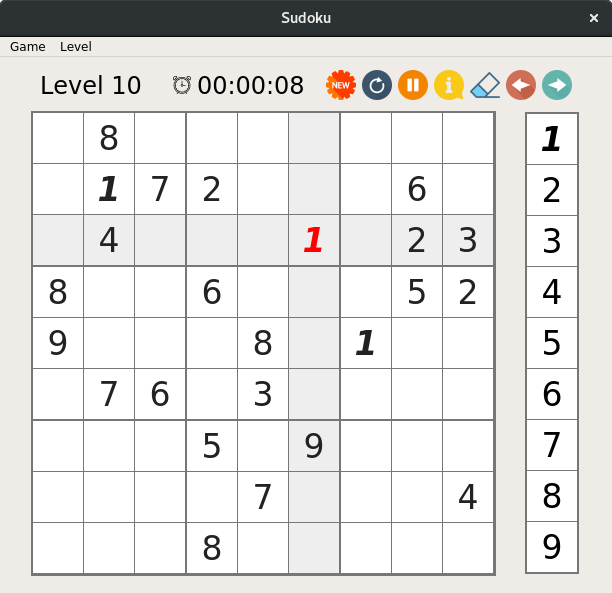
\includegraphics[width=\linewidth]{sudoku-3c.png}
		\caption{最高难度的数独} \label{fig:sudoku-3c}
	\end{subfigure}

	\vspace{0.5cm}
	\begin{subfigure}{.45\textwidth}
		\centering
		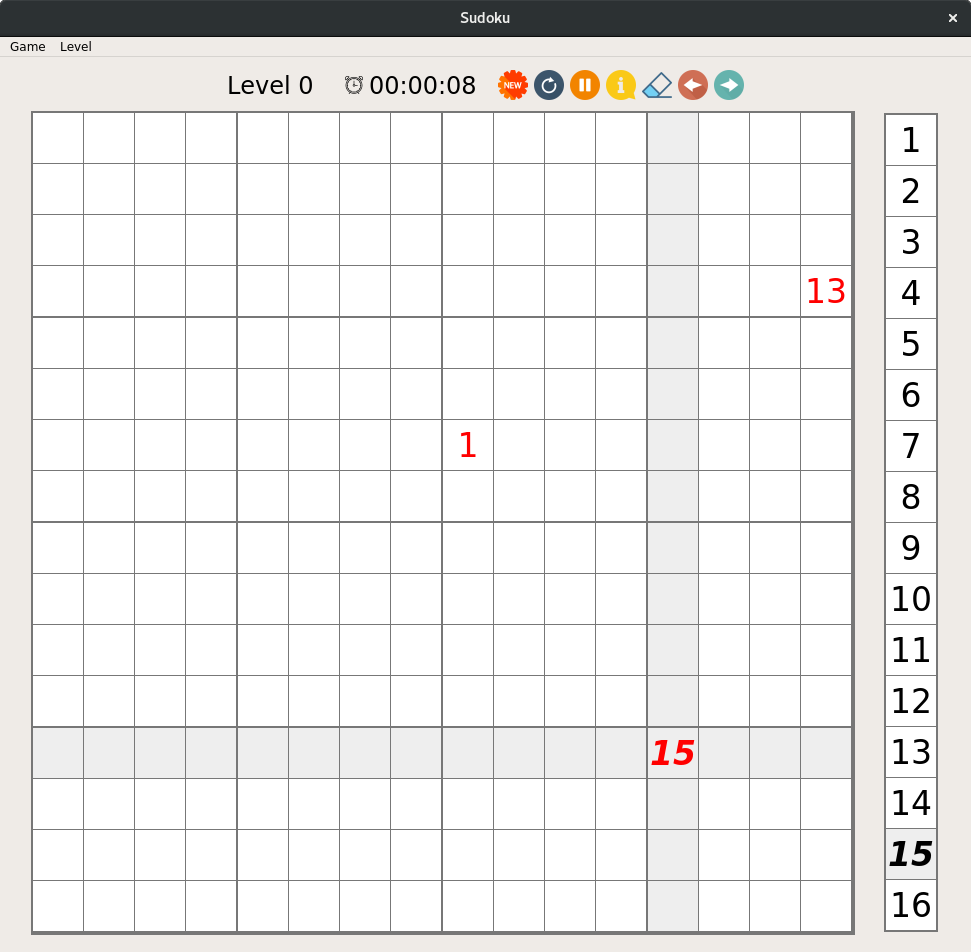
\includegraphics[width=\linewidth]{sudoku-4c.png}
		\caption{一个玩家任意输入的游戏} \label{fig:sudoku-4c}
	\end{subfigure}
	\hfill
	\begin{subfigure}{.45\textwidth}
		\centering
		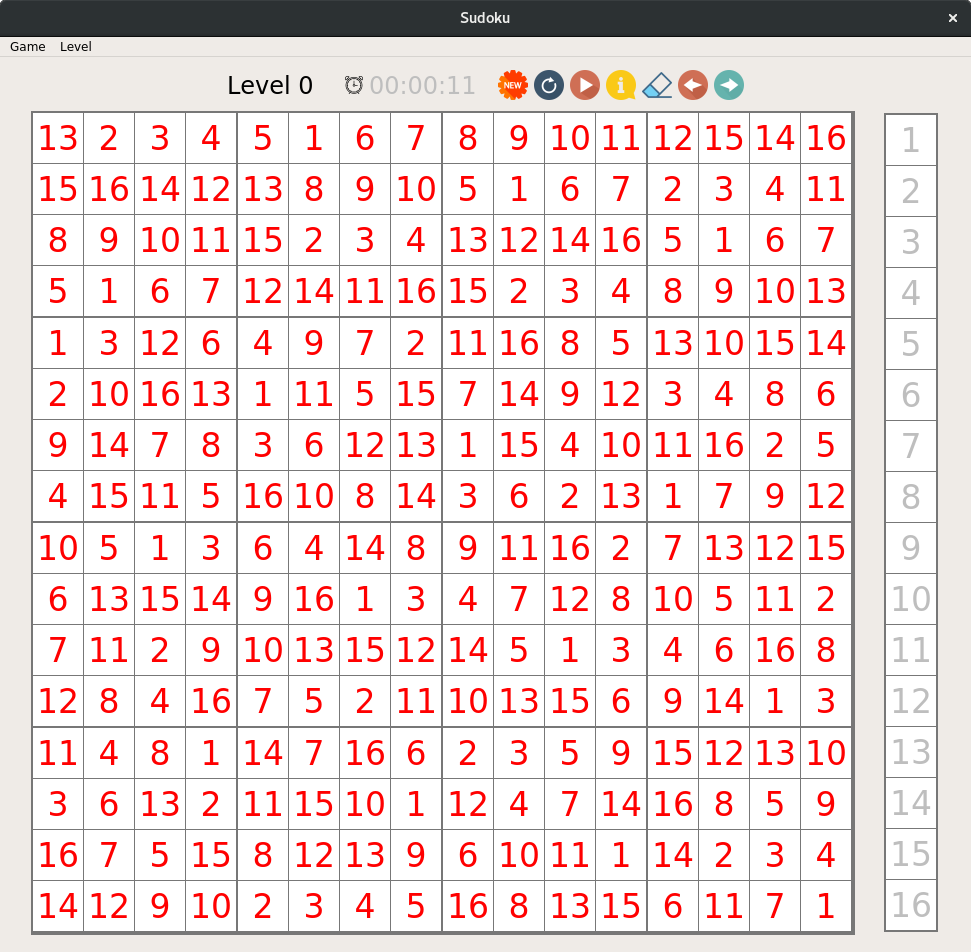
\includegraphics[width=\linewidth]{sudoku-4d.png}
		\caption{利用算法计算出的答案} \label{fig:sudoku-4d}
	\end{subfigure}
	\caption{(\subref{fig:sudoku-3b}, \subref{fig:sudoku-3c})上方的按钮从左到右分别为:新游戏、重完、暂停/开始、提示、清除、撤销和取消撤销。黑色的数字表示初始时题目所给出的数字,大号红色数字表示用户已经确定的数字,小号红色数字表示候选的数字。当前选中的格子以及与其所在相同行或列的格子被高亮显示,同时右侧数字栏中已经选择的数字被加粗显示,可以方便进行操作。另外,对于已经确定的数字,其余与其相同并且也已经确定的数字会被加粗显示,如(\subref{fig:sudoku-3c})。玩家对于重要的数字可以进行标记,标记为在格子左上角打上一个三角(例如(\subref{fig:sudoku-3b})中的数字3)。}
\end{figure}

玩家在空格中填入的数字分为确定数(采用正常大小的字体表示)以及候选数(采用小号字体表示)。确定数只能存在一个,候选数可以存在多个,并且确定数和候选数不能同时存在。

玩家可以通过多种方式进行格子的选择:
\begin{itemize}
	\item 通过鼠标直接点击格子进行选中。
	\item 通过键盘方向键来进行当前选中格子的切换。
	\item 通过Tab键快速切换到下一个格子。
\end{itemize}

玩家可以用鼠标右键点击格子来对其进行标记。

玩家在选中一个格子之后,如果该格子的数字已经确定,那么所有与该数相同的数将会被加粗显示,以方便确认是否满足数独的条件。同时,所有与该格在相同行或列的格子都会被高亮显示。此外,无论该格子数字确定与否,右侧数字列表中该格子的所有数都会被加粗。

玩家可以通过多种方式在空格中填入数字:
\begin{itemize}
	\item 通过键盘直接输入数字将填入对应的确定数,如果Ctrl键被按下,那么填入的将会是候选数。
	\item 通过鼠标点击右侧数字列表填入。使用鼠标左键点击将会填入确定数,右键点击则会填入候选数。
\end{itemize}

玩家也可以通过多种方式在空格中填入数字:
\begin{itemize}
	\item 通过键盘删除键删除格子中的一个数字。
	\item 通过鼠标点击右侧数字列表已经选中的数进行删除。
	\item 通过“清除”功能键来清除该格子所有的数字。
\end{itemize}
\section{难度选择算法}
我们认为一个数独游戏的难度可以根据行列空格数的最大值以及给定数字的数量来确定。行列空格数的最大值越小玩家拥有的信息量就越多,同样给定数字越多玩家也能获得更多的信息。

在我们的难度中,最简单的关卡给出的数字至少有50个,并且行列空格数不会超过4个。然而,在最困难的关卡中,最少只会给出20个数字,并且可能会有某些行或列全部是空格。在最简单和最困难中间这两个影响难度的因素平滑过渡。

为了生成一个满足条件的数独,可以按照以下步骤来实现:

\begin{enumerate}
	\item 在空白棋盘随机填入数十个数。
	\item 利用求解算法获得一个合法解,如果不存在合法解,转到1。
	\item 生成一个随机的格子排列。
	\item 按照这个序列来尝试一个个删除所填入的数字,如果删除后能保证解唯一并且满足之前的条件,那么就删除,否则不删除。
	\item 如果删除了足够的数字,则返回。否则跳到1。
\end{enumerate}

为了实现快速的数独问题求解,我们利用Dancing Link来优化搜索。
\section{GUI部分实现细节}
主要的游戏棋盘是通过$3\times 3$的QGridLayout,每个QGridLayout里再套一个$3\times 3$的QGridLayout来实现的。

功能按钮的鼠标移入以及点击的效果是通过QPainter::drawImage里图片的混合选项来实现的,通过多次混合以及不同的混合参数就可以实现颜色的深浅变化:

\begin{minted}{c++}
void ToolButton::paintEvent(QPaintEvent *)
{
    QPainter p(this);
    QPixmap bg(image_path);
    p.drawPixmap(QPoint(0, 0), bg);
    if(is_mouse_pressed)
    {
        p.setCompositionMode(QPainter::CompositionMode_Multiply);
        p.drawPixmap(QPoint(0, 0), bg);
    } else if(is_mouse_over) {
        p.setCompositionMode(QPainter::CompositionMode_HardLight);
        p.drawPixmap(QPoint(0, 0), bg);
    }
}
\end{minted}

另外,关于窗口大小的固定,由于在切换数独棋盘大小时窗口大小也会随之改变,可以利用{\it minimumSizeHint()}来直接进行计算:

\begin{minted}{c++}
    setFixedSize(window->minimumSizeHint()
               + ui->menuBar->minimumSizeHint());
\end{minted}
\end{document}
